\documentclass[10pt]{NSP1}
\usepackage{url,floatflt}
\usepackage{helvet,times}
\usepackage{psfig,graphics}
\usepackage{mathptmx,amsmath,amssymb,bm}
\usepackage{float}
\usepackage[bf,hypcap]{caption}
\usepackage{keyval}
\makeatletter
\define@key{psfig}{file}{\def\psfig@file{#1}}
\define@key{psfig}{width}{\def\psfig@width{#1}}
\define@key{psfig}{height}{\def\psfig@height{#1}}
\renewcommand{\psfig}[1]{%
  \let\par\@@par%
  \setkeys{psfig}{#1}%
  \includegraphics[width=3.6truecm,height=5truecm,keepaspectratio]{\psfig@file}%
}
\renewenvironment{biographyps}[2]{%
  \begingroup
  \endgraf
  \skip0=0pt plus2cm
  \advance\skip0 by2\bigskipamount\relax
  \vskip\skip0
  \small
  \setbox0=\vbox\bgroup%
                 \sloppy
                 \noindent
                 \hangindent=113pt
                 \hangafter=-14\relax
                 \smash{\raise 6.5pt
                        \llap{\vbox to0pt{\psfig{#1}%
                                          \vss}\kern11pt}}%
                 \if!#2!\else{\sc\ignorespaces#2\/} \fi
                 \ignorespaces
}{%
  \egroup
  \dimen0=\ht0\advance\dimen0 by\dp0
  \ifdim\dimen0<5cm
     \vtop to5cm{\box0\vss}
  \else
     \box0
  \fi
  \par\addvspace{12pt}%
  \endgroup
}
\makeatother

\addtolength{\oddsidemargin}{.5in}
\addtolength{\evensidemargin}{-.5in}

\tolerance=1
\emergencystretch=\maxdimen
\hyphenpenalty=10000
\hbadness=10000

\topmargin=0.00cm

\def\sm{\smallskip}
\def\no{\noindent}

\def\firstpage{1}
\setcounter{page}{\firstpage}
\def\thevol{11}
\def\thenumber{3}
\def\theyear{2022}

\begin{document}

\titlefigurecaption{{\large \bf \rm Journal of Statistics Applications \& Probability}\\ {\it\small An International Journal}}

\title{Statistical Analysis of Body Dysmorphic Disorder, Quality of Life, and Social Anxiety in Fire Victims: Path Analysis}

\author{Abdallah Almahaireh \and Baha' Shawaqfeh \and Bahaa Eldeen Abu Serdaneh^{1}}
\institute{$^{1}$ Ph.D. in Educational Psychology, School of Educational Science, The University of Jordan.}
\received{25 Nov}
\revised{4 Jan}
\accepted{15 Jan}
\published{1 ---}

\abstracttext{The study aimed to explore the relationship between body dysmorphic disorder symptoms and quality of life, and the role of social anxiety disorder symptoms among fire victims. The study used a quantitative technique using path analysis. The study sample consists of 292 participants. The study used body dysmorphic disorder symptoms, quality of life, and social anxiety disorder symptoms scales. The results showed that there is a moderate level of quality of life among fire victims while there is a High level of body dysmorphic disorder symptoms and social anxiety symptoms. Also, the results show that social anxiety disorder symptoms have moderate role in the relationship between body dysmorphic disorder symptoms and quality of life among fire victims. On the other hand, body dysmorphic disorder symptoms influence quality of life through one path which is indirect mediated by social anxiety disorder symptoms. The model explains 46\% of quality of life. The study concludes that this result should be considered when specialists need to improve the quality of life among fire victims by addressing the negative body dysmorphic and focusing on their social anxiety symptoms. This may help them improve their mental health and wellness.}

\keywords{Body Dysmorphic, Quality of Life, Social Anxiety, Fire Victims.}

\maketitle

\section{1 Introduction}

Fires is one of the common causes for injuries and death globally, which occur 180 thousand annually. In Jordan 21999 patients visits burn unit in governmental hospital . There is a lack of interest in burning injuries which need a long-term treatment which may happen to anyone, anywhere, and anytime. Burning May be caused by many factors such as gas, electricity, and hot water which result psychological and physical problems resulting decreasing in Quality of life (QOL) among fire victims.

QOL is affected by many variables related to burning such as; the response to injury, speed treatment response, quality of treatment, social support, and counselling . The QOL is defined as “the individual’s perception of their position in life in the context of culture and value systems in which they live and in relation to their goals, expectations, standards, and concerns” .

QOL is an extent of individual’s awareness of the experiences and how much he’s satisfied with his basic need fulfillment in life. Also, how much they feel happiness, accomplishment, and integration in terms of psychological, physical, cognitive, social, and emotional health . Fire victim’s QOL is affected by many aspects. Gautam et al.,  study found that burn injuries has a negative impact on QOL and its domains; psychology, physically, socially, and environmentally.

Fires harm the body physically and leads to marks and deformities which affect the individual’s body image. Fire victims could be experience body dysmorphic disorder symptoms (BDDS) that is defined as a disorder caused by a body defect in the external appearance that can be seen by others or can’t be seen. How the individual sees him self is very important because it develops his perception of self and how much he’s acceptable to others , the burning marks can lead the person to be not satisfied of his body and they know that others can see it which leads him to avoid social situations .

The social anxiety disorder symptoms (SADS) refers to a high level of anxiety happened when the individual faces social engagement and it leads him to avoid any interaction with others also it effects his life socially, occupationally, or on other functional areas . This can be affected negatively on their quality of life and leads them to isolation. Especially when they review the negative situations they have been exposed to, then evaluate them and create a negative thought about it, this affect their professional and social performance. It’s an important matter for the individual to feel healthy and psychologically wellbeing.

The best way to investigates these relations is by using path analysis method which is a statistical method investigate the direct, indirect, and total effects by mediating variable between at least two variables and it’s an extension method of multiple regression . This method helps in to test the theoretical model which assumed in this study that the SADS mediating the relationship between BDDS and QOL.

This study focused on how the BDDS can affect QOL, and if the SADS has a moderate role between them among fire victims. We believe that because of the body deformities that shows on fire victims it may increase BDDS this leads them to avoid social interactions and expressed SADS that affects negatively on many functional areas related to the QOL. The suggested model shown in figure 1.

Figure 1: The suggested model for relationship between BDDS and QOL and the moderating of SADS

1.1 Research questions

What is the level of the BDDS, QOL, and SADS among fire victims?

Is there a relationship between BDDS, QOL, and SADS among fire victims?

Do the SADS moderate the relationship between BDDS and QOL among fire victims?

\begin{enumerate}
  \item Materials and Methods
\end{enumerate}

2.1 Study design

This research employs a quantitative technique using path analyses. A volunteer selected 305 fire victims those who survived the burning from the Dermatology Clinics in Jordan from 2020 to 2025. The inclusion criteria for this study were: (1) accepted to by in this research, (2) exposure to the burning between 2020 and 2025, (3) the burning is effect on main parts like face, nick, and hands who usually don’t cover them, (4) who shows that the burning affect their life. as subjects; all participants supplied written informed permission with the scales. The research ethics committee authorized the institution’s study.

2.2 Participants

The study sample consists of 292 fire victims from the Dermatology Clinic in Jordan from 2020 to 2025. The distribution of participants by socioeconomic rank is as follows: 100 Male and 190 females. 137 were single and 153 were married. Their age was between 18-50 with a mean of (33.6 ±8.9).

2.3 Data collection Tools

2.3.1 Body Dysmorphic Disorder Symptoms Scale

The researchers used a scale of  items from Al-Hasi . Participants rated each item on a four-Likert scale, from 1 (Strongly disagree) to 4 (Strongly agree). The researcher extracted the validity and reliability and found that the discriminate evidence ranged between 0.344 and 0.713. Cronbach’s alpha was 0.914.

2.3.2 Social Anxiety Disorder Symptoms Scale

The researchers used a scale of 10 items from Shawaqfeh \& Almahaireh . Participants rated each item on a four-Likert scale, from 1 (Strongly disagree) to 4 (Strongly agree). The researcher extracted the validity and reliability and found that the discriminate evidence ranged between 0.478 and 0.915. Cronbach’s alpha was 0.916.

2.3.3 Quality of Life Scale

The researchers used a scale of 24 items from Abu Al-wafaa . It’s including 4 dimensions (Physical, Psychological, Social Relationships, Environmental). Participants rated each item on a four-Likert scale, from 1 (Never) to 4 (Always). The researcher extracted the validity and reliability and found that the discriminate evidence ranged between 0.345 and 0.922. Cronbach’s alpha was ranged between 0.737-0.918.

2.4 Data collection

The researchers obtained approval for this study from the Institutional Review Board at Al-Ahliyya Amman University. The registration number 467/2025/1. The date was 17/6/2025. Anonymized data was collected by the researchers, the survey was conducted by paper instruments, the first page contain the purpose and the significance of the study.

2.5 Data analysis

The researchers entered the data into SPSS data sheet, and used IBM SPSS Statistics for Windows, version 27 to analyze the data. Means, standard deviations, Pearson’s correlation were calculated. Also, IBM SPSS AMOS v24 was used to do the path analyses, the missing data were filled using SPSS program using series mean method in replace missing values, this procedure used because AMOS don’t calculate any data with missing values.

Path analysis used to examine and explore the relationships between the observed variables (BDDS, SADS, QOL). This technique is used to test the link between two variables via a third variable. Because of that it considered as a complex technique than multiple regression analysis. The advantage of sing it is its superior ability to detect relationships and it studied many variables at the same time .

\begin{enumerate}
  \item Findings
\end{enumerate}

3.1 The level of the BDDS, QOL, and SADS

To investigate the level of the BDDS, QOL, and SADS among fire victims. Means and standard deviations were calculated. Table 1 show that the level of the QOL among fire victims was moderate with a mean of (2.29±0.169). While the levels of BDDS and SADS was high with a means of (3.14±0.568) for the BDDS and (3.08±0.704) for the SADS.

\begin{table}[htbp]
\centering
\resizebox{\linewidth}{!}{%
\begin{tabular}{cccc}
\hline
Variable & Mean & Std. & Level \\
\hline
BDDS & 3.14 & .568 & High \\
QOL & 2.29 & .169 & Moderate \\
SADS & 3.08 & .704 & High \\
\hline
\end{tabular}%
}
\caption{}

\end{table}

Table 1: Means and standard deviations of the BDDS, QOL, and SADS

3.2 The relationship between BDDS, QOL, and SADS

To investigate the relationship between BDDS, QOL, and SADS among fire victims. Person correlation coefficients were calculated. Table 2 that there is statistically significant negative relationship between QOL and each of BDDS and SADS (R= -.626 and -0.644). While there is statistically significant positive relationship between BDDS and SADS (R= .675).

\begin{table}[htbp]
\centering
\resizebox{\linewidth}{!}{%
\begin{tabular}{cccccc}
\hline
Correlation & Sig. & Correlation & Sig. & Correlation & Sig. \\
\hline
BDDS & - & - & -.626* & .000 & .675* & .000 \\
QOL & - & - & - & - & -.644* & .000 \\
SADS & - & - & - & - & - & - \\
\hline
\end{tabular}%
}
\caption{}

\end{table}

** sig at the 0.01 level (2-talied)

Table 2: Person correlation test results between BDDS, QOL, and SADS

3.3 Examination of the moderating effect of SADS

To examine if SADS has a moderate effect in the relationship between BDDS and QOL among fire victims, path analyses were computed using SPSS AMOS V24. The assumptions were checked by checking the normality distribution. The results in table 3 and the figures 2-4 show that the variables are normally distributed which the Skewness ranged between .398 and -.945, while the Kurtosis ranged between -.745 and .954 .

\begin{table}[htbp]
\centering
\resizebox{\linewidth}{!}{%
\begin{tabular}{cccc}
\hline
Statistic & Std. Error & Statistic & Std. Error \\
\hline
BDDS & -.945 & .143 & .789 & .285 \\
QOL & .398 & .143 & .954 & .285 \\
SADS & -.426 & .143 & -.745 & .285 \\
\hline
\end{tabular}%
}
\caption{}

\end{table}

Table 3: Means and standard deviations of the BDDS, QOL, and SADS

\begin{figure}[htbp]
\centering
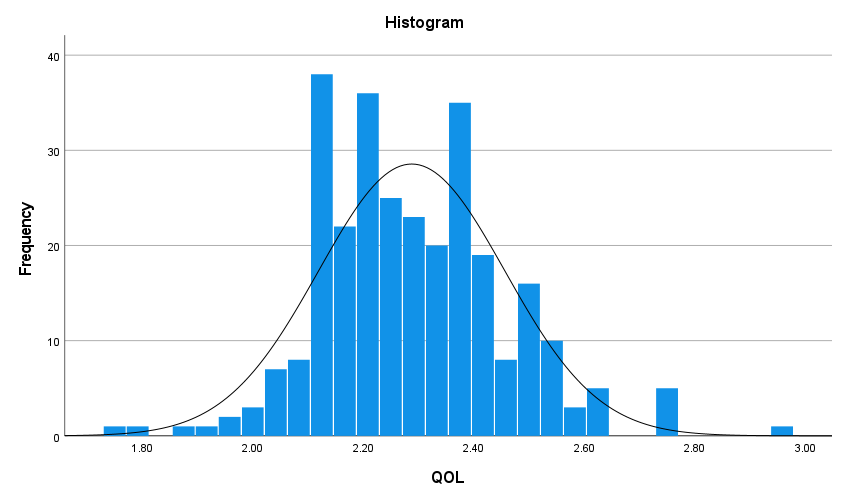
\includegraphics[width=\linewidth,height=0.3\textheight,keepaspectratio]{media/image5.png}
\caption{}

\end{figure}

Figure 2: The normally distribution of the QOL

It’s appears from figure 2 that the QOL is normally distributed which the histogram show that the values ranged between 1 to 3. While the most values ranged between 2.1 to 2.6 and it’s appears that there are normal distribution.

\begin{figure}[htbp]
\centering
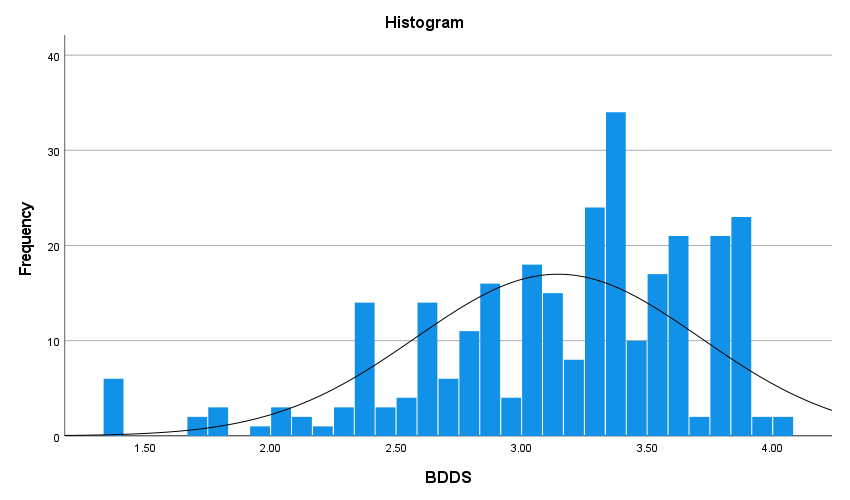
\includegraphics[width=\linewidth,height=0.3\textheight,keepaspectratio]{media/image6.png}
\caption{}

\end{figure}

Figure 3: The normally distribution of the BDDS

It’s appears from figure 3 that the BDDS is normally distributed which the histogram show that the values ranged between 1.4 to 4. While the most values ranged between 2.4 to 3.9 and it’s appears that there are normal distribution.

\begin{figure}[htbp]
\centering
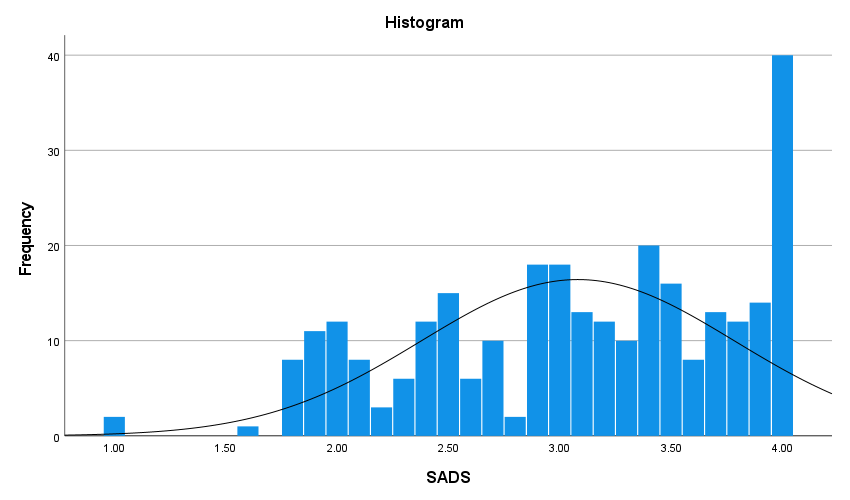
\includegraphics[width=\linewidth,height=0.3\textheight,keepaspectratio]{media/image7.png}
\caption{}

\end{figure}

Figure 4: The normally distribution of the SADS

It’s appears from figure 4 that the SADS is normally distributed which the histogram show that the values ranged between 1 to 3. While the most values ranged between 1.7 to 4 and it’s appears that there is normal distribution.

Also, the model fit parameters were checked in table 4. The results show that the model is fit due to the CMIN/df=2.428, RMSEA= 0.069, and CFI= 0.739 according to Hair et al. .

\begin{table}[htbp]
\centering
\resizebox{\linewidth}{!}{%
\begin{tabular}{ccc}
\hline
Model fit parameters & Value & Acceptable value \\
\hline
CMIN/df & 2.428 & Less than 5 \\
RMSEA & 0.069 & Less than 0.1 \\
CFI & 0.739 & Greater than 0.7 \\
\hline
\end{tabular}%
}
\caption{}

\end{table}

Table 4: Model fit parameters

In figure 5 the results show that SADS has moderate role in the relationship between BDDS and QOL among fire victims. According to table 5 BDDS influence QOL through one path which is indirect mediated by SADS. Although, there are positive direct effect of BDDS on SADS achieves .459, and negative direct effect of SADS on QOL achieves -.654. On the other hand, the direct effect of BDDS on QOL was quietly low (-.049) but the indirect effect was significant and negative which was -.300.

\begin{figure}[htbp]
\centering
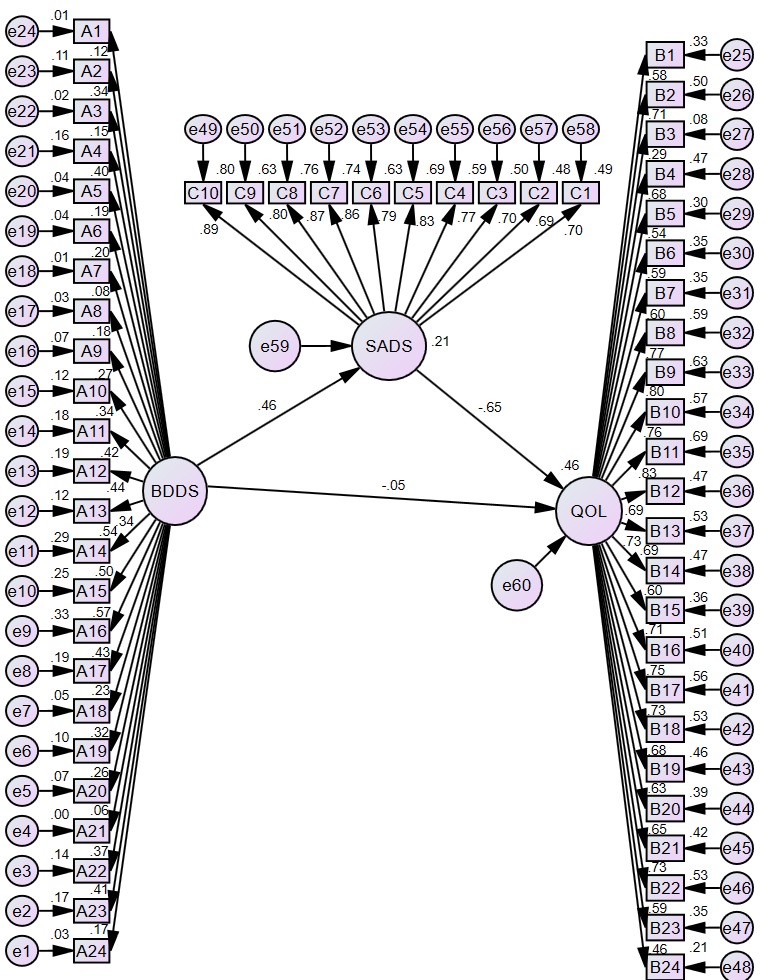
\includegraphics[width=\linewidth,height=0.3\textheight,keepaspectratio]{media/image8.png}
\caption{}

\end{figure}

Figure 5: The tested model for relationship between BDDS and QOL and the moderating of SADS

\begin{table}[htbp]
\centering
\resizebox{\linewidth}{!}{%
\begin{tabular}{ccccc}
\hline
Independent & Dependent & Direct effect & Indirect effect & Total effect \\
\hline
BDDS & SADS & .459 & - & .459 \\
BDDS & QOL & -.049 & -.300 & -.349 \\
SADS & QOL & -.654 & - & -.654 \\
\hline
\end{tabular}%
}
\caption{}

\end{table}

Table 5: Direct, indirect, and Total effects between the variables

After the results showed that SADS has moderate role in the relationship between BDDS and QOL among fire victims. The square multiple regression in the model was investigate. As shown in table 6 the model explains 21.1\% from SADS and 46\% from QOL. It is a good weight of prediction.

\begin{table}[htbp]
\centering
\resizebox{\linewidth}{!}{%
\begin{tabular}{cc}
\hline
Variable & Estimate \\
\hline
SADS & .211 \\
QOL & .460 \\
\hline
\end{tabular}%
}
\caption{}

\end{table}

Table 6: square multiple regression for SADS and QOL in the model

\begin{enumerate}
  \item Discussion
\end{enumerate}

The results of this study show that the SADS has a moderate role in the relationship between BDDS and QOL among fire victims. Thus, the BDDS has only indirect effect through the SADS but the direct effect in the model was very low despite that the correlation between them was significant and negative -.626. On the other hand, the fire victims have a moderate level of QOL and High level of SADS and BDDS.

These results show that the burn increases the BDDS, makes the person think others will not accept them, and look at them negatively. they focus on how others will judge them, and they feel humiliated when others look at them because of their burn marks . SADS makes QOL decrease because it affects how they deals with others and tries to avoid them, leading them to stay alone . Also, they may avoid going to their workplace because they feel ashamed and fears how others will assess them and their burn marks , which affect their occupational and social QOL. Emotionally, they suffered from negative feelings, pessimism, and low self-esteem related to the negative thinking about their body .

Usually, fire victims struggled with others, such as when others look at them intently or appear afraid. This means that self-perception is the most important factor in how BDDS affect QOL. If the fire victims feel afraid from others staring at them and think that their burns are a stigma, they will suffer from SADS, which leads them to avoidance and depression overall; this will decrease QOL.

The Strengths of this study are its the first research study the relations BDDS, QOL, SADS. Used the path analyses and structural equation model to investigate the SADS as a moderate variable between BDDS and QOL. The results was very impressive in this study especially that when SADS moderate the relationship between BDDS and QOL it canceled the direct impact and change it to indirect impact even though the relation was -.626 which consider high correlation value.

We believe that this study can be improved by entering other variables in the model such as self-talk between BDDS and SADS, or self-perception which we think that it has a good impact on QOL. Also, the researcher should consider compare the fire victims with other participants to make sure if these results applied on them or all how had Body deformity and focus on compare between the individuals who had Body deformity from birth and who’s involved in an accident.

\begin{enumerate}
  \item Conclusions
\end{enumerate}

In conclusion, we believe that the model has proved a good explanation for the effect of BDDS on QOL through SADS. It should be considered in future research and when specialists need to improve the quality of life among fire victims by addressing the negative body dysmorphic and focusing on their social anxiety symptoms. This may help them improve their mental health and wellness. Further studies could investigate the self-esteem, self-perception, and social self-efficacy.

Data Availability:

The datasets analyzed during the current study are available from the corresponding author upon reasonable request.

Conflict of Interest:

The authors declare no conflicts of interest in this study.

Funding:

This research received no specific grants from funding agencies.

Consent to Participate:

Participants provided informed consent to participate in this study.

Ethics approval:

This study followed the principles of the Committee on Publication Ethics (COPE).

\begin{thebibliography}{99}
\bibitem{ref1}
World Health Organization (WHO) (2023). Burns. Available from:

\bibitem{ref2}
Jordanian Ministry of Health (MOH) (2025). Annual statistically report for 2024.

\bibitem{ref3}
Hunt JL, Arnoldo BD, Purdue GF. Chapter 4—prevention of burn injuries. Total burn care. 7th ed. London: WB Saunders. 2012:47‑55.

\bibitem{ref4}
Ho, J. H. (2024). University of Washington quality of life questionnaire. In Encyclopedia of Quality of Life and Well-Being Research (pp. 7398-7400). Cham: Springer International Publishing.

\bibitem{ref5}
Al-Harthi, I. \& Al-Samadi, A. (2017). The level of health behavior among Umm Al-Qura University students: A descriptive study, Educational Journal, 31 (122), 125-145.

\bibitem{ref6}
Gautam, R., Rajoura, O. P., Sharma, A. K., \& Bhatia, M. S. (2022). Socio-demographic features and quality of life post burn injury. Journal of family medicine and primary care, 11(3), 1032-1035.

\bibitem{ref7}
Rück, C., Mataix-Cols, D., Feusner, J. D., Shavitt, R. G., Veale, D., Krebs, G., \& Fernández de la Cruz, L. (2024). Body dysmorphic disorder. Nature Reviews Disease Primers, 10(1), 92.

\bibitem{ref8}
Sreshta, N., Pope, H. G., Hudson, J. I., \& Kanayama, G. (2017). Muscle dysmorphia. Body dysmorphic disorder: advances in research and clinical practice, 81.

\bibitem{ref9}
Alhammadi, A. (2020). Overview of the Diagnostic and Statistical Manual of Mental Disorders, Alarabia for science.

\bibitem{ref10}
American Psychiatric Association. (2013). Diagnostic and statistical manual of mental disorders (DSM-5®). American Psychiatric Pub.

\bibitem{ref11}
Columbia (2026). Path Analysis. Available from: .

\bibitem{ref12}
Al-Hasi, D. (2023). Body Dysmorphic Disorder and Body Esteem and the Relationship to Self-Harm among a Sample of Patients in Cosmetic Clinics. Unpublished Master Thesis, Al-Ahliyya Amman University.

\bibitem{ref13}
Shawaqfeh, B. \& Almahaireh, A. (). Social Anxiety Disorder Symptoms among Divorced Women in Amman and the Differences in It According to Some Demographic Variables. Al-Quds Open University Journal For Research, 13 (38), 87-96.

\bibitem{ref14}
Abu Al-wafaa, A. (2024). The Relationship Between Social Anxiety and Quality of Life Among Sample of Psychiatric Clinic Clients in Amman: a Comparative Correlation Study. Unpublished Master Thesis. The University of Jordan.

\bibitem{ref15}
Garson, G. D. (2014). Path analysis (2 ed.). Asheboro, NC: Statistical Associates Publishing.

\bibitem{ref16}
Hair, J. F., Black, W. C., Babin, B., Anderson, R. E., \& Tatham, R. (2018). Multivariate data analysis: Cengage.

\bibitem{ref17}
Suluhan, D., SAĞIROĞLU, E., Demir, S., YILDIZ, D., Onat, M., \& Şenel, E. (2023). Determination of the relationship between self-esteem and social anxiety in adolescents with burns. Türkiye Çocuk Hastalıkları Dergisi, 1-7.

\bibitem{ref18}
Gorbani, A., Rezaiee Moradali, M., \& Shabanloei, R. (2021). Relationship between self‐esteem and perceived social support in burn patients in Sina Hospital of Tabriz. Nursing open, 8(3), 1194-1200.

\bibitem{ref19}
Hussain, M., Tariq, M., \& Hussain, M. (2023). Social appearance anxiety, psychological distress and quality of life among patients with burn injuries. Journal of Professional \& Applied Psychology, 4(3), 418-428.

\bibitem{ref20}
Yeşilyurt, İ., \& Kendirkıran, G. (2024). The effect of social appearance anxiety and body perception on the quality of life in burn patients. International Wound Journal, 21(2), e14720.

\bibitem{ref21}


\end{thebibliography}


\begin{biographyps}{file=media/image9.jpeg}{Abdallah Almahaireh}
Abdallah Almahaireh is Counselling and Special Education Department, School of Educational Science, The University of Jordan. He received the Ph.D. degree in Educational and Psychological Counselling at The University of Jordan.\end{biographyps}

\begin{biographyps}{file=media/image10.jpeg}{Baha' Shawaqfeh}
Baha' Shawaqfeh is Full-time lecturer in Counselling and Mental Health Department, Faculty of Educational Science, The World Islamic Sciences and Education University. He received the Ph.D. degree in Educational and Psychological Counselling at The University of Jordan.\end{biographyps}

\begin{biographyps}{file=media/image11.jpeg}{Bahaa Eldeen Abu Serdaneh}
Bahaa Eldeen Abu Serdaneh has a Ph.D. degree in Educational Psychology, School of Educational Science, at The University of Jordan.\end{biographyps}

\begin{biography}{Authors Biography}
Authors Biography\end{biography}



\end{document}
